\documentclass[11pt]{amsart}

\usepackage[T1]{fontenc}
\usepackage{lmodern}
\usepackage{amssymb}
\usepackage{mathtools}
\usepackage{microtype}
\usepackage{booktabs}
\usepackage{xcolor}
\usepackage{float}
\usepackage{tikz}
\usetikzlibrary{arrows.meta,calc,positioning}
\usepackage{url}
\usepackage{hyperref}

\makeatletter
\g@addto@macro\UrlBreaks{\do\_\do\.}
\makeatother

\setlength{\emergencystretch}{3em}
\hypersetup{
  colorlinks=true,
  linkcolor=blue!55!black,
  citecolor=green!40!black,
  urlcolor=blue!55!black,
  pdftitle={Peripheral Benzel Tilings with Right Stones and Three Bone Orientations},
  pdfauthor={Alex Chengyu Li}
}

\newtheorem{theorem}{Theorem}[section]
\newtheorem{proposition}[theorem]{Proposition}
\newtheorem{lemma}[theorem]{Lemma}
\newtheorem{corollary}[theorem]{Corollary}
\theoremstyle{definition}
\newtheorem{definition}[theorem]{Definition}
\newtheorem{remark}[theorem]{Remark}

\newcommand{\Bz}{\mathcal B}
\newcommand{\cT}{\mathcal T}
\newcommand{\CT}{\operatorname{CT}}

\title[Peripheral benzel tilings]
{Peripheral Benzel Tilings with Right Stones\\
and Three Bone Orientations}

\author{Alex Chengyu Li}
\address{Independent Researcher, Tokyo, Japan; ORCID 0009-0008-4516-8946}
\email{cl7076@nyu.edu}
\date{August 2026}
\dedicatory{\normalfont\small\textbf{Formalization status.}
A kernel-only Lean~4 formalization of the results in this manuscript has been
completed using Mathlib, with no project-specific axioms.}

\subjclass[2020]{Primary 05A15, 05B45; Secondary 05A10}
\keywords{benzel tilings, trihexes, lattice paths, ballot paths,
multivariate Lagrange inversion}

\begin{document}

\begin{abstract}
Propp asked for the number of tilings of the peripheral benzel
$\Bz(n,2n-3)$ by right stones and all three orientations of bones.  We prove
his conjectured formula
\[
 T_{103}(n,2n-3)
 =\frac{(3n+3)(3n-7)!}{(n-5)!(2n-1)!}\qquad(n\geq5).
\]
The proof first partitions the hexagonal cells into periodic three-cell
owners.  A linear owner-label energy forces every stone to occupy one owner
and every bone to become a label-preserving directed edge.  The edge set is
then a directed $Y$: three paths from the deficient corner owners to one
interior sink, with no other common vertices.  At a fixed sink, the two
last-edge chiralities reduce to independent one-dimensional ballot counts; in
one chirality, three adjacent-binomial factors cancel cyclically.  A
three-variable constant-term evaluation followed by Lagrange inversion gives
the stated formula.
\end{abstract}

\maketitle

\section{Introduction}

Benzels are threefold-symmetric regions in the hexagonal grid introduced by
Propp as finite regions for exact trimer enumeration
\cite{ProppProblems}.  The five relevant trihexes are two triangular
\emph{stones} and three collinear \emph{bones}.  Write $T_{ijk}(a,b)$ for
the number of tilings of the $(a,b)$-benzel when right stones are allowed if
$i=1$, left stones are allowed if $j=1$, and $k$ bone orientations are
allowed.

Several of Propp's problems have been solved using abacus and compression
bijections \cite{DLPY,DFLPY}.  Those methods are particularly effective when
at least one bone orientation is forbidden.  The present problem permits all
three bone orientations and lies on the peripheral diagonal $b=2a-3$.
Propp states the following as Problem~6 and reports verification for
$5\leq n\leq16$ \cite{ProppProblems}.  Propp's online status table, whose
most recent problem update is dated June 2025, still listed Problem~6 as open
when accessed on 22 August 2026 \cite{ProppSite}.

\begin{theorem}[Propp's Problem 6]\label{thm:main}
For every integer $n\geq5$,
\[
 T_{103}(n,2n-3)
 =\frac{(3n+3)(3n-7)!}{(n-5)!(2n-1)!}.
\]
\end{theorem}

The proof uses a periodic right-stone tiling to partition the plane into
three-cell owners.  Although the benzel has quadratic area, the
Conway--Lagarias invariant and an owner-label energy force every admissible
tiling to differ from this periodic background along only three directed
paths.  These paths have total length $3n-6$ and meet at a single interior
owner.  The rest of the proof enumerates the three-path configurations.

Put $m=n-5$.  The conjectured number has the useful ballot form
\begin{equation}\label{eq:ballot-form}
 2\binom{3m+8}{m}-\binom{3m+8}{m-1}
 =\frac{3(m+6)}{2m+9}\binom{3m+8}{m}.
\end{equation}
The path reduction explains both terms: one sink chirality gives a cyclically
telescoping product of binomial counts, while the other gives ballot counts.

\section{Benzels, stones, and bones}

Represent a hexagonal cell center by $(i,j)\in\mathbb Z^2$ and put
$k=1-i-j$.  This is the barycentric convention used by Propp
\cite{ProppProblems}.  The $(a,b)$-benzel is the cell set
\[
 \Bz(a,b)=\left\{(i,j):
 -(a-1)\leq j-i,\ k-j,\ i-k\leq b-1\right\}.
\]
The right stone is the translate class of
\[
 R=\{(0,0),(1,0),(0,1)\},
\]
and the three bones have direction sets
\[
\begin{aligned}
 H&=\{(0,0),(1,0),(2,0)\},\\
 V&=\{(0,0),(0,1),(0,2)\},\\
 D&=\{(0,0),(1,-1),(2,-2)\}.
\end{aligned}
\]
Only translates, not rotations beyond these three listed bone types, are
used.

The area and Conway--Lagarias invariant give the following tile counts
\cite{ConwayLagarias,ProppProblems}.

\begin{lemma}\label{lem:tile-counts}
Every type-$103$ tiling of $\Bz(n,2n-3)$ has
\[
 \frac{(n-5)(n-2)}2
 \quad\hbox{right stones and}\quad
 3(n-2)\quad\hbox{bones}.
\]
\end{lemma}

\begin{proof}
Substitution in the benzel area formula gives
\[
 |\Bz(n,2n-3)|=\frac{3(n-2)(n+1)}2,
\]
so a tiling has $(n-2)(n+1)/2$ trihexes.  Since no left stones are allowed,
the Conway--Lagarias invariant equals the number of right stones.  Its
$a+b\equiv0\pmod3$ formula at $(a,b)=(n,2n-3)$ is
\[
 \frac{3(a-b)^2-a-b}{6}
 =\frac{(n-5)(n-2)}2.
\]
Subtracting from the total number of trihexes gives $3(n-2)$ bones.
\end{proof}

\section{Periodic owners and the energy certificate}

Put $t=n-2$ and work modulo three.  An \emph{owner anchor} is a pair
$(q,r)$ with
\[
 q-r\equiv t\pmod3.
\]
The anchor owns the three cells
\[
 (q,r),\qquad(q+1,r),\qquad(q,r+1),
\]
labelled $0,1,2$, respectively.  Every cell of the infinite hexagonal grid
has a unique owner: among its three possible right-stone anchors, the three
values of $q-r$ represent the three residue classes.

For an owner anchor $(q,r)$ define
\begin{equation}\label{eq:owner-coordinates}
 u=\frac{t-q+r}{3},\qquad
 v=\frac{t-q-2r}{3},\qquad
 w=\frac{t+2q+r}{3}.
\end{equation}
These are integers with $u+v+w=t$.

\begin{lemma}[Owner simplex]\label{lem:owner-simplex}
The owners meeting $\Bz(n,2n-3)$ are in bijection with
\[
 \Delta_t=\{(u,v,w)\in\mathbb N_0^3:u+v+w=t\}.
\]
Every non-corner owner contributes all three of its cells to the benzel.  The
three corner owners contribute two cells each: $(0,t,0)$ misses label $0$,
$(0,0,t)$ misses label $1$, and $(t,0,0)$ misses label $2$.
\end{lemma}

\begin{proof}
For a cell $(i,j)$ put $k=1-i-j$ as above.  Substitution of the three labels
at $(q,r)$ gives the following ordered triples
$(j-i,k-j,i-k)$:
\[
\begin{array}{c|ccc}
\text{label}&j-i&k-j&i-k\\ \hline
0&3u-t&3v-t+1&3w-t-1\\
1&3u-t-1&3v-t&3w-t+1\\
2&3u-t+1&3v-t-1&3w-t.
\end{array}
\]
The benzel bounds are $-t-1\leq j-i,k-j,i-k\leq2t$.  If any one of the
three cells lies in the benzel, its row in the table, together with the
integrality of $u,v,w$, forces $u,v,w\geq0$.  Conversely, suppose
$u,v,w\geq0$ and $u+v+w=t$.  The table then shows
\begin{align*}
 \text{label }0\text{ is present}&\iff v<t,\\
 \text{label }1\text{ is present}&\iff w<t,\\
 \text{label }2\text{ is present}&\iff u<t.
\end{align*}
The inverse coordinate change is
\[
 q=w-u,\qquad r=u-v;
\]
indeed $q-r=t-3u\equiv t\pmod3$.  Thus every owner meeting the benzel
corresponds to a unique point of $\Delta_t$, and every point of $\Delta_t$
contributes at least two cells.
A coordinate can equal $t$ only when the other two coordinates vanish.  The
three such points give exactly the three missing labels stated in the lemma;
all other owners contribute all three cells.
\end{proof}

At anchor $(q,r)$ give labels $0,1,2$ the respective integer energies
\begin{equation}\label{eq:cell-energy}
 h_0(q,r)=q+r,\qquad h_1(q,r)=-q,\qquad h_2(q,r)=-r.
\end{equation}

\begin{lemma}[Local energy table]\label{lem:energy-table}
Relative to the owner phase above, the four possible tile classes have the
following energies.
\begin{center}
\begin{tabular}{lcc}
\toprule
tile class & number of owners & energy\\
\midrule
in-phase right stone & $1$ & $0$\\
wrong-phase right stone & $3$ & $3$\\
two-owner bone & $2$ & $1$\\
three-owner bone & $3$ & $4$\\
\bottomrule
\end{tabular}
\end{center}
For a two-owner bone, the owner containing two cells is its source.  The label
missing at the source equals the label of the single target cell.
\end{lemma}

\begin{proof}
For an in-phase stone, the three energies at one owner sum to zero.  The
remaining cases depend only on the translation class modulo three.  For a
translate based at $(i,j)$, put
\[
 \rho\equiv i-j-t\pmod3,\qquad \rho\in\{0,1,2\}.
\]
Direct substitution in \eqref{eq:cell-energy} gives
\[
\begin{array}{c|cccc}
\rho& R&H&V&D\\ \hline
0&0&1&1&1\\
1&3&4&1&4\\
2&3&1&4&1.
\end{array}
\]
Here the entry for $R$ at $\rho=0$ is the in-phase stone.  The six
energy-one bone cases have the following source-missing label and directed
owner displacement:
\[
\begin{array}{c|cc}
\text{bone and phase}&\text{label}&\text{step}\\ \hline
(H,0)&2&A\\
(H,2)&2&B\\
(V,0)&1&C\\
(V,1)&1&B\\
(D,0)&0&C\\
(D,2)&0&A.
\end{array}
\]
In every row, the two source cells are precisely the two labels other than
the displayed one, and the target cell has the displayed label.  Hence its
energy is $-h_\ell(\text{source})+h_\ell(\text{target})=1$.  The three
unlisted bone phases meet three owners and have energy four, which completes
the table.
\end{proof}

\begin{proposition}[Energy rigidity]\label{prop:energy-rigidity}
Every right stone in a type-$103$ tiling of $\Bz(n,2n-3)$ is in phase, and
every bone is a two-owner, label-preserving directed edge.
\end{proposition}

\begin{proof}
Every full owner has total energy zero.  At each corner the two present labels
have total energy $t$, so Lemma~\ref{lem:owner-simplex} gives total benzel
energy $3t=3(n-2)$.

Let $s$ be the number of wrong-phase stones and $f$ the number of three-owner
bones.  Lemma~\ref{lem:tile-counts} gives $3(n-2)$ bones.  Of these,
$3(n-2)-f$ have energy one and $f$ have energy four, while the $s$
wrong-phase stones have energy three.  The total tile energy is therefore
\[
 [3(n-2)-f]+4f+3s=3(n-2)+3(s+f).
\]
Comparison with the benzel energy gives $s+f=0$, hence $s=f=0$.
\end{proof}

\section{The directed \texorpdfstring{$Y$}{Y}}

In anchor coordinates, the only directed displacements are
\[
 A=(2,-1),\qquad B=(-1,-1),\qquad C=(-1,2).
\]
In simplex coordinates they are
\begin{align*}
 A&:(u,v,w)\longmapsto(u-1,v,w+1),\\
 B&:(u,v,w)\longmapsto(u,v+1,w-1),\\
 C&:(u,v,w)\longmapsto(u+1,v-1,w).
\end{align*}
Label $0$ permits $A,C$, label $1$ permits $B,C$, and label $2$ permits
$A,B$.  The corresponding potential $h_\ell$ increases by one on every
edge carrying label $\ell$.  We replace each bone by the directed edge from
its two-cell owner to its one-cell owner; the second table in the proof of
Lemma~\ref{lem:energy-table} shows that this correspondence is unique in both
directions.

\begin{proposition}[Directed-$Y$ bijection]\label{prop:Y-bijection}
Type-$103$ tilings of $\Bz(n,2n-3)$ are in bijection with triples of labelled
paths in $\Delta_t$ satisfying the following conditions.
\begin{enumerate}
\item The paths of labels $0,1,2$ start at $(0,t,0)$, $(0,0,t)$, and
      $(t,0,0)$, respectively.
\item Each path uses its two permitted steps, and the vertex sets of two
      different paths intersect only at their common endpoint.
\item The paths have one common endpoint $(u,v,w)$ with $u,v,w>0$.
\end{enumerate}
Every full owner outside the three paths is occupied by a right stone.
\end{proposition}

\begin{proof}
An outgoing edge uses two cells of its source owner, whereas an incoming edge
uses one cell of its target owner.  At a full owner not occupied by a stone,
let $o$ and $i$ denote the numbers of outgoing and incoming edges.  Exact
coverage gives $2o+i=3$, and two outgoing edges would overlap.  Hence either
$(o,i)=(1,1)$ or $(o,i)=(0,3)$.  In the first case the incoming edge covers
the label omitted by the outgoing edge, so both carry the same label.  In the
second case the incoming labels are $0,1,2$.  At a deficient corner the same
argument gives $2o+i=2$: either there is one outgoing edge carrying the
missing label, or there are two incoming edges carrying the two present
labels.

Since $|\Delta_t|=\binom{t+2}{2}=\binom n2$, Lemma~\ref{lem:tile-counts}
leaves
\[
 \binom n2-\frac{(n-5)(n-2)}2=3t+1
\]
owners not occupied by stones.  There are $3t$ bone edges.  If $K$ is the
number of full three-incoming sinks and $P$ the number of two-incoming corner
sinks, every other active owner has one outgoing edge.  Counting outgoing
edges therefore gives
\[
 3t=(3t+1)-K-P,
\]
so $K+P=1$.

No directed cycle is possible because the constant label potential strictly
increases along every edge of a pass-through component.  It remains to rule
out $P=1$.  By cyclic symmetry suppose $(0,t,0)$ is the corner sink.  A
label-$1$ path from $(0,0,t)$ to this corner uses only $B$-steps: $B$ leaves
$u$ unchanged, $C$ increases it, and both endpoints have $u=0$.  Its vertex
set is therefore
\[
 \{(0,b,t-b):0\leq b\leq t\}.
\]
A label-$2$ path from $(t,0,0)$ to the same corner must use exactly $t$
$A$-steps and $t$ $B$-steps.  Immediately after its final $A$-step it is at
$(0,b,t-b)$ for some $b<t$; equality $b=t$ would make the preceding
$w$-coordinate negative.  This vertex belongs to the label-$1$ path and is
not the common corner sink, contradicting the local coverage rules.  Hence
$K=1$ and $P=0$.

Following outgoing edges from the three corners now gives the required three
paths.  They cannot meet before the unique sink: a pass-through owner has only
one incoming edge, and the sink already has its three incoming labels.  Their
common endpoint is a full owner and therefore has three positive simplex
coordinates.  Any further component would have no sink and hence, by
finiteness, would contain a directed cycle.

Conversely, replace every permitted labelled step by the unique bone from
Lemma~\ref{lem:energy-table}.  At a source, the outgoing bone covers the two
present labels.  At a pass-through owner, the incoming bone covers the path
label and the outgoing bone covers the other two labels.  At the common sink,
the three incoming bones cover labels $0,1,2$.  In-phase stones cover every
unused full owner.  The intersection condition ensures that these local
coverings are compatible, so they form a unique tiling.
\end{proof}

Write the sink as
\[
 (u,v,w)=(x+1,y+1,z+1),\qquad x+y+z=m=n-5.
\]
At the sink the last directions must be distinct, since equal directions
would give the same predecessor owner to two paths.  Respecting the two
allowed directions for each label leaves exactly two possibilities:
\[
 (+):(C,B,A),\qquad (-):(A,C,B)
\]
for labels $(0,1,2)$.

\begin{figure}[H]
\centering
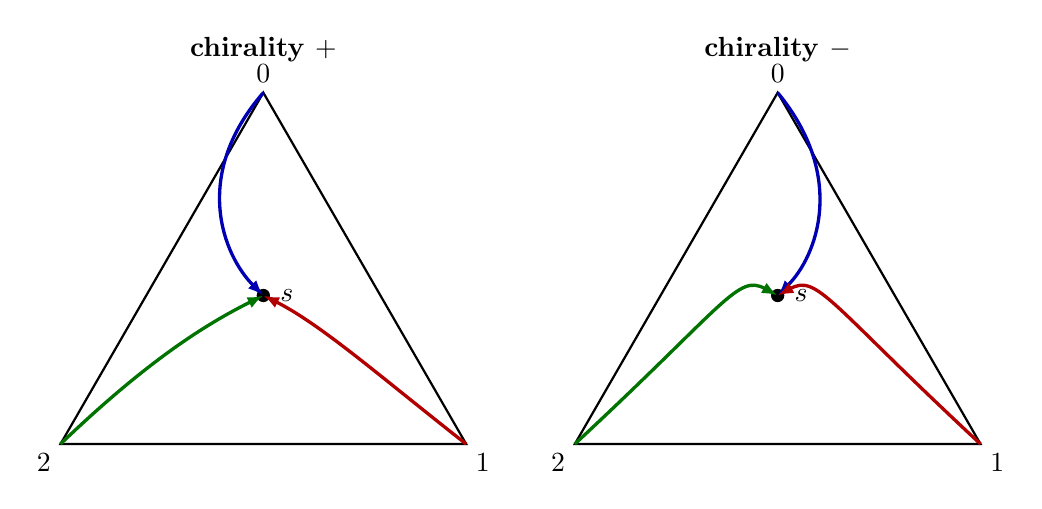
\begin{tikzpicture}[scale=0.92,>=Latex,
  pzero/.style={very thick,blue!70!black,-{Latex[length=2mm]}},
  pone/.style={very thick,red!70!black,-{Latex[length=2mm]}},
  ptwo/.style={very thick,green!45!black,-{Latex[length=2mm]}}]
\foreach \dx/\sgn in {0/1,7.1/-1}{
  \begin{scope}[xshift=\dx cm]
    \coordinate (L) at (-2.8,-1.8);
    \coordinate (R) at (2.8,-1.8);
    \coordinate (T) at (0,3.05);
    \coordinate (S) at (0,0.25);
    \draw[thick] (L)--(R)--(T)--cycle;
    \node[below left] at (L) {$2$};
    \node[below right] at (R) {$1$};
    \node[above] at (T) {$0$};
    \node[circle,fill=black,inner sep=1.7pt,label=right:$s$] at (S) {};
    \ifnum\sgn=1
      \draw[pzero] (T) .. controls (-1.0,1.9) and (-0.55,0.8) .. (S);
      \draw[pone] (R) .. controls (1.65,-0.9) and (0.8,-0.15) .. (S);
      \draw[ptwo] (L) .. controls (-1.6,-0.65) and (-0.8,-0.15) .. (S);
    \else
      \draw[pzero] (T) .. controls (0.95,1.9) and (0.55,0.8) .. (S);
      \draw[pone] (R) .. controls (0.7,0.15) and (0.55,0.55) .. (S);
      \draw[ptwo] (L) .. controls (-0.7,0.15) and (-0.55,0.55) .. (S);
    \fi
    \node[font=\bfseries] at (0,3.65)
      {chirality \ifnum\sgn=1 $+$\else $-$\fi};
  \end{scope}
}
\end{tikzpicture}
\caption{The three labelled arms, the fixed sink, and the two possible
last-edge chiralities.  The drawing is schematic; the proof uses the simplex
coordinates.}
\label{fig:chiralities}
\end{figure}

\section{Fixed-sink enumeration}

Put
\[
 N_x=2x+y+2,\qquad N_y=2y+z+2,\qquad N_z=2z+x+2,
\]
and adopt the convention $\binom N{-1}=0$.

\begin{lemma}[Independent arms]\label{lem:independent-arms}
Fix the sink $(x+1,y+1,z+1)$ and one of the two last-edge chiralities.
Any three individually admissible labelled arms with those endpoints and last
edges intersect only at the sink.  The numbers of choices for the arms of
labels $(0,1,2)$ are, respectively,
\begin{align*}
 (+):\quad&
 \binom{N_z}{z+1}-\binom{N_z}{z},\quad
 \binom{N_x}{x+1}-\binom{N_x}{x},\quad
 \binom{N_y}{y+1}-\binom{N_y}{y},\\
 (-):\quad&
 \binom{N_z}{z}-\binom{N_z}{z-1},\quad
 \binom{N_x}{x}-\binom{N_x}{x-1},\quad
 \binom{N_y}{y}-\binom{N_y}{y-1}.
\end{align*}
\end{lemma}

\begin{proof}
The step multiplicities from the three sources to the sink are
\[
\begin{array}{c|cc}
\text{label}&\multicolumn{2}{c}{\text{step multiplicities}}\\ \hline
0&A:z+1&C:x+z+2\\
1&B:x+y+2&C:x+1\\
2&A:y+z+2&B:y+1.
\end{array}
\]
For label $0$, the only nontrivial simplex constraint along the path is
$u\geq0$, or equivalently that every prefix contains at least as many
$C$-steps as $A$-steps.  For labels $1$ and $2$, the corresponding conditions
are, respectively, at least as many $B$-steps as $C$-steps and at least as
many $A$-steps as $B$-steps.  Remove the prescribed last step.  The reflection
principle for a word with $k$ minority letters gives
$\binom Nk-\binom N{k-1}$: reflecting the initial segment ending at the first
negative prefix bijects the bad words with the words having $k-1$ minority
letters.  This yields the six displayed counts.

It remains to check that independently chosen arms cannot meet prematurely.
Every vertex on the label-$0$, label-$1$, and label-$2$ arms satisfies,
respectively,
\[
 v\geq y+1,\ w\leq z+1;\qquad
 w\geq z+1,\ u\leq x+1;\qquad
 u\geq x+1,\ v\leq y+1.
\]
Thus a common vertex of arms $0$ and $1$ must lie on $w=z+1$.  In positive
chirality the final $B$-step of arm $1$ is its first arrival at this boundary;
in negative chirality the final $A$-step of arm $0$ is its first arrival.
Hence the two arms meet only at the sink.  The same argument on the boundaries
$u=x+1$ and $v=y+1$, cyclically, separates the other two pairs.  This proves
both independence and the stated arm counts.
\end{proof}

\begin{corollary}\label{cor:fixed-sink}
Let $P(x,y,z)$ and $Q(x,y,z)$ denote the positive- and negative-chirality
counts at the fixed sink.  Then
\begin{align}
 P(x,y,z)
 &=\prod_{\mathrm{cyc}}\binom{2x+y+2}{x},\label{eq:Pxyz}\\
 Q(x,y,z)
 &=\prod_{\mathrm{cyc}}
 \left(\binom{2x+y+2}{x}-\binom{2x+y+2}{x-1}\right).\label{eq:Qxyz}
\end{align}
In particular,
\begin{equation}\label{eq:QoverP}
 \frac{Q(x,y,z)}{P(x,y,z)}
 =\frac{(x+3)(y+3)(z+3)}
 {(x+y+3)(y+z+3)(z+x+3)}.
\end{equation}
\end{corollary}

\begin{proof}
The negative-chirality product in Lemma~\ref{lem:independent-arms} is exactly
\eqref{eq:Qxyz}.  For $N=2r+s+2$,
\[
 \binom N{r+1}-\binom Nr
 =\frac{s+1}{r+1}\binom Nr.
\]
Applying this identity to the three positive-chirality factors gives the
additional multiplier
\[
 \frac{x+1}{z+1}\frac{y+1}{x+1}\frac{z+1}{y+1}=1,
\]
which proves \eqref{eq:Pxyz}.  Finally,
\[
 \frac{\binom{2r+s+2}{r}-\binom{2r+s+2}{r-1}}
      {\binom{2r+s+2}{r}}
 =\frac{s+3}{r+s+3}.
\]
Multiplying its three cyclic instances gives \eqref{eq:QoverP}.
\end{proof}

\section{Summing the sinks}

Define
\[
 P(t)=\sum_{x,y,z\geq0}P(x,y,z)t^{x+y+z},\qquad
 Q(t)=\sum_{x,y,z\geq0}Q(x,y,z)t^{x+y+z}.
\]

\begin{proposition}\label{prop:generating-functions}
Let $T=T(t)$ be the unique formal power series satisfying
\[
 T=1+tT^3.
\]
Then
\begin{align}
 P(t)&=\frac{T^9}{(3-2T)(T^2-3T+3)},\label{eq:Pgf}\\
 Q(t)&=(2-T)^3P(t),\label{eq:Qgf}\\
 P(t)+Q(t)&=T^9\frac{3-T}{3-2T}.\label{eq:Ygf}
\end{align}
\end{proposition}

\begin{proof}
Use
\[
 \binom{2x+y+2}{x}=[a^x](1+a)^{2x+y+2}
\]
and its cyclic analogues in \eqref{eq:Pxyz}.  Summing three geometric series
gives \eqref{eq:constant-term}: the powers of $x$, for example, form the
geometric ratio $t(1+a)^2(1+c)/a$.  Thus
\begin{equation}\label{eq:constant-term}
 P(t)=\CT_{a,b,c}
 \frac{(1+a)^2(1+b)^2(1+c)^2}{D_aD_bD_c},
\end{equation}
where
\begin{align*}
 D_a&=1-\frac{t(1+a)^2(1+c)}a,\\
 D_b&=1-\frac{t(1+b)^2(1+a)}b,\\
 D_c&=1-\frac{t(1+c)^2(1+b)}c.
\end{align*}
We evaluate this formal constant term by the multivariate Lagrange--Good
residue formula \cite{Good}.  Its small-root equations are
\[
 a=t(1+a)^2(1+c),\quad
 b=t(1+b)^2(1+a),\quad
 c=t(1+c)^2(1+b).
\]
They have a unique solution in $t\mathbb Q[[t]]^3$: once all coefficients
below degree $d$ are known, the equations determine the degree-$d$
coefficients.  Cyclic symmetry therefore gives $a=b=c=U$, where
$U=t(1+U)^3$; put $T=1+U$.

At the small root, put
\[
 r=\frac UT=\frac{T-1}{T},\qquad
 d=1-2r=\frac{2-T}{T}.
\]
For $\phi_a=(1+a)^2(1+c)$ and its cyclic analogues, the Good denominator is
the determinant of
\[
 \left(\delta_{ij}-\frac{x_j}{\phi_i}
 \frac{\partial\phi_i}{\partial x_j}\right)_{i,j\in\{a,b,c\}}.
\]
At the small root this matrix and its determinant are
\[
 J=\begin{pmatrix}d&0&-r\\-r&d&0\\0&-r&d\end{pmatrix},
 \qquad
 \det J=d^3-r^3
 =\frac{(3-2T)(T^2-3T+3)}{T^3}.
\]
The numerator in \eqref{eq:constant-term} becomes $T^6$.  Division by the
determinant contributes the additional factor $T^3$, proving
\eqref{eq:Pgf}.

The ballot identity
\[
 \binom Nk-\binom N{k-1}=[a^k](1-a)(1+a)^N
\]
with $\binom N{-1}=0$ shows that the constant term for $Q(t)$ has the additional numerator
$(1-a)(1-b)(1-c)$.  At the small root this is $(1-U)^3=(2-T)^3$, proving
\eqref{eq:Qgf}.  Finally,
\[
 1+(2-T)^3=(3-T)(T^2-3T+3),
\]
which gives \eqref{eq:Ygf}.
\end{proof}

\begin{proof}[Proof of Theorem~\ref{thm:main}]
Differentiating $T=1+tT^3$ and simplifying \eqref{eq:Ygf} gives
\[
 P(t)+Q(t)=2T^9+\frac13t\frac{d}{dt}T^9.
\]
Hence
\[
 [t^m](P(t)+Q(t))=\frac{m+6}{3}[t^m]T^9.
\]
The ordinary Lagrange inversion formula yields
\[
 [t^m]T^9=\frac9{2m+9}\binom{3m+8}{m}.
\]
For $m=0$ this is immediate; for $m>0$ it follows from
\[
 [t^m](1+U)^9=\frac9m[u^{m-1}](1+u)^{3m+8}.
\]
Consequently
\[
 [t^m](P(t)+Q(t))
 =\frac{3(m+6)}{2m+9}\binom{3m+8}{m}.
\]
The adjacent-binomial identity
\[
 \binom{3m+8}{m-1}=\frac{m}{2m+9}\binom{3m+8}{m}
\]
gives \eqref{eq:ballot-form}.  Substituting $m=n-5$ proves
Theorem~\ref{thm:main}.
\end{proof}

\section{Computational checks}

A direct exact-cover program implements the barycentric benzel and the
four permitted prototile classes directly.  It reproduces the formula for
$5\leq n\leq11$ and records the owner graph of every tiling.  A separate
directed-path program verifies the fixed-sink chirality products and the total
formula through $n=12$.  These computations are finite consistency checks and
are not used in the proof of Theorem~\ref{thm:main}.

A kernel-only Lean~4 formalization defines the literal benzel and prototiles,
proves the tile-count invariant and tiling/path equivalence, and verifies the
generating-function and closed-form steps.  Its exact 19-label map compiles with
\texttt{--trust=0}; the endpoints use only \texttt{propext},
\texttt{Classical.choice}, and \texttt{Quot.sound}.  The finite computations
above remain independent consistency checks rather than formal premises.

\paragraph{Data and code availability.}
The complete formalization and reproducibility files are available in the
\href{https://github.com/crabsatellite/peripheral-benzel-tilings}{public code
repository}; versioned releases are archived through Zenodo.

\section*{Declaration of generative AI and AI-assisted technologies in the
manuscript preparation process}

During the preparation of this work, the author used OpenAI Codex and an
author-developed local research system to assist with proof exploration,
programming, formalization, and language editing.  The author reviewed the
resulting mathematical statements, computations, citations, and prose and
takes full responsibility for the content of the manuscript.

\section*{Statements and declarations}

\paragraph{Competing interests.}
The author declares no known competing financial or non-financial interests
that are directly or indirectly related to this work.

\paragraph{Funding.}
No funding was received for conducting this study or preparing the manuscript.

\paragraph{Acknowledgements.}
The author thanks the developers of Lean and Mathlib for the formalization
environment.

\enlargethispage{8\baselineskip}
\bibliographystyle{amsplain}
\bibliography{references}

\end{document}
